\pdfoutput=1
%% Author: PGL  Porta Mana
%% Created: 2015-05-01T20:53:34+0200
%% Last-Updated: 2020-03-17T16:56:56+0100
%%%%%%%%%%%%%%%%%%%%%%%%%%%%%%%%%%%%%%%%%%%%%%%%%%%%%%%%%%%%%%%%%%%%%%%%%%%%
\newif\ifarxiv
\arxivfalse
\ifarxiv\pdfmapfile{+classico.map}\fi
\newif\ifafour
\afourtrue% true = A4, false = A5
\newif\iftypodisclaim % typographical disclaim on the side
\typodisclaimfalse
\newcommand*{\memfontfamily}{zplx}
\newcommand*{\memfontpack}{newpxtext}
\documentclass[\ifafour a4paper,12pt,\else a5paper,10pt,\fi%extrafontsizes,%
onecolumn,oneside,article,%french,italian,german,swedish,latin,
british%
]{memoir}
\newcommand*{\firstdraft}{16 March 2020}
\newcommand*{\firstpublished}{16 March 2020}
\newcommand*{\updated}{\ifarxiv***\else\today\fi}
\newcommand*{\propertitle}{Sketch of replies to N. Comp. reviews%\\{\large ***}%
}% title uses LARGE; set Large for smaller
\newcommand*{\pdftitle}{\propertitle}
\newcommand*{\headtitle}{}
\newcommand*{\pdfauthor}{}
\newcommand*{\headauthor}{}
\newcommand*{\reporthead}{}%\ifarxiv\else Open Science Framework \href{https://doi.org/10.31219/osf.io/***}{\textsc{doi}:10.31219/osf.io/***}\fi}% Report number

%%%%%%%%%%%%%%%%%%%%%%%%%%%%%%%%%%%%%%%%%%%%%%%%%%%%%%%%%%%%%%%%%%%%%%%%%%%%
%%% Calls to packages (uncomment as needed)
%%%%%%%%%%%%%%%%%%%%%%%%%%%%%%%%%%%%%%%%%%%%%%%%%%%%%%%%%%%%%%%%%%%%%%%%%%%%

%\usepackage{pifont}

%\usepackage{fontawesome}

\usepackage[T1]{fontenc} 
\input{glyphtounicode} \pdfgentounicode=1

\usepackage[utf8]{inputenx}

%\usepackage{newunicodechar}
% \newunicodechar{Ĕ}{\u{E}}
% \newunicodechar{ĕ}{\u{e}}
% \newunicodechar{Ĭ}{\u{I}}
% \newunicodechar{ĭ}{\u{\i}}
% \newunicodechar{Ŏ}{\u{O}}
% \newunicodechar{ŏ}{\u{o}}
% \newunicodechar{Ŭ}{\u{U}}
% \newunicodechar{ŭ}{\u{u}}
% \newunicodechar{Ā}{\=A}
% \newunicodechar{ā}{\=a}
% \newunicodechar{Ē}{\=E}
% \newunicodechar{ē}{\=e}
% \newunicodechar{Ī}{\=I}
% \newunicodechar{ī}{\={\i}}
% \newunicodechar{Ō}{\=O}
% \newunicodechar{ō}{\=o}
% \newunicodechar{Ū}{\=U}
% \newunicodechar{ū}{\=u}
% \newunicodechar{Ȳ}{\=Y}
% \newunicodechar{ȳ}{\=y}

\newcommand*{\bmmax}{0} % reduce number of bold fonts, before font packages
\newcommand*{\hmmax}{0} % reduce number of heavy fonts, before font packages

\usepackage{textcomp}

%\usepackage[normalem]{ulem}% package for underlining
% \makeatletter
% \def\ssout{\bgroup \ULdepth=-.35ex%\UL@setULdepth
%  \markoverwith{\lower\ULdepth\hbox
%    {\kern-.03em\vbox{\hrule width.2em\kern1.2\p@\hrule}\kern-.03em}}%
%  \ULon}
% \makeatother

\usepackage{amsmath}

\usepackage{mathtools}
\addtolength{\jot}{\jot} % increase spacing in multiline formulae
\setlength{\multlinegap}{0pt}

%\usepackage{empheq}% automatically calls amsmath and mathtools
%\newcommand*{\widefbox}[1]{\fbox{\hspace{1em}#1\hspace{1em}}}

%%%% empheq above seems more versatile than these:
%\usepackage{fancybox}
%\usepackage{framed}

% \usepackage[misc]{ifsym} % for dice
% \newcommand*{\diceone}{{\scriptsize\Cube{1}}}

\usepackage{amssymb}

\usepackage{amsxtra}

\usepackage[main=british,french,italian,german,swedish,latin,esperanto]{babel}\selectlanguage{british}
\newcommand*{\langfrench}{\foreignlanguage{french}}
\newcommand*{\langgerman}{\foreignlanguage{german}}
\newcommand*{\langitalian}{\foreignlanguage{italian}}
\newcommand*{\langswedish}{\foreignlanguage{swedish}}
\newcommand*{\langlatin}{\foreignlanguage{latin}}
\newcommand*{\langnohyph}{\foreignlanguage{nohyphenation}}

\usepackage[autostyle=false,autopunct=false,english=british]{csquotes}
\setquotestyle{british}

\usepackage{amsthm}
\newcommand*{\QED}{\textsc{q.e.d.}}
\renewcommand*{\qedsymbol}{\QED}
\theoremstyle{remark}
\newtheorem{note}{Note}
\newtheorem*{remark}{Note}
\newtheoremstyle{innote}{\parsep}{\parsep}{\footnotesize}{}{}{}{0pt}{}
\theoremstyle{innote}
\newtheorem*{innote}{}

\usepackage[shortlabels,inline]{enumitem}
\SetEnumitemKey{para}{itemindent=\parindent,leftmargin=0pt,listparindent=\parindent,parsep=0pt,itemsep=\topsep}
% \begin{asparaenum} = \begin{enumerate}[para]
% \begin{inparaenum} = \begin{enumerate*}
\setlist{itemsep=0pt,topsep=\parsep}
\setlist[enumerate,2]{label=\alph*.}
\setlist[enumerate]{label=\arabic*.,leftmargin=1.5\parindent}
\setlist[itemize]{leftmargin=1.5\parindent}
\setlist[description]{leftmargin=1.5\parindent}
% old alternative:
% \setlist[enumerate,2]{label=\alph*.}
% \setlist[enumerate]{leftmargin=\parindent}
% \setlist[itemize]{leftmargin=\parindent}
% \setlist[description]{leftmargin=\parindent}

\usepackage[babel,theoremfont,largesc]{newpxtext}

\usepackage[bigdelims,nosymbolsc%,smallerops % probably arXiv doesn't have it
]{newpxmath}
\linespread{1.083}%\useosf
%% smaller operators for old version of newpxmath
\makeatletter
\def\re@DeclareMathSymbol#1#2#3#4{%
    \let#1=\undefined
    \DeclareMathSymbol{#1}{#2}{#3}{#4}}
%\re@DeclareMathSymbol{\bigsqcupop}{\mathop}{largesymbols}{"46}
%\re@DeclareMathSymbol{\bigodotop}{\mathop}{largesymbols}{"4A}
\re@DeclareMathSymbol{\bigoplusop}{\mathop}{largesymbols}{"4C}
\re@DeclareMathSymbol{\bigotimesop}{\mathop}{largesymbols}{"4E}
\re@DeclareMathSymbol{\sumop}{\mathop}{largesymbols}{"50}
\re@DeclareMathSymbol{\prodop}{\mathop}{largesymbols}{"51}
\re@DeclareMathSymbol{\bigcupop}{\mathop}{largesymbols}{"53}
\re@DeclareMathSymbol{\bigcapop}{\mathop}{largesymbols}{"54}
%\re@DeclareMathSymbol{\biguplusop}{\mathop}{largesymbols}{"55}
\re@DeclareMathSymbol{\bigwedgeop}{\mathop}{largesymbols}{"56}
\re@DeclareMathSymbol{\bigveeop}{\mathop}{largesymbols}{"57}
%\re@DeclareMathSymbol{\bigcupdotop}{\mathop}{largesymbols}{"DF}
%\re@DeclareMathSymbol{\bigcapplusop}{\mathop}{largesymbolsPXA}{"00}
%\re@DeclareMathSymbol{\bigsqcupplusop}{\mathop}{largesymbolsPXA}{"02}
%\re@DeclareMathSymbol{\bigsqcapplusop}{\mathop}{largesymbolsPXA}{"04}
%\re@DeclareMathSymbol{\bigsqcapop}{\mathop}{largesymbolsPXA}{"06}
\re@DeclareMathSymbol{\bigtimesop}{\mathop}{largesymbolsPXA}{"10}
%\re@DeclareMathSymbol{\coprodop}{\mathop}{largesymbols}{"60}
%\re@DeclareMathSymbol{\varprod}{\mathop}{largesymbolsPXA}{16}
\makeatother
%%
%% With euler font cursive for Greek letters - the [1] means 100% scaling
\DeclareFontFamily{U}{egreek}{\skewchar\font'177}%
\DeclareFontShape{U}{egreek}{m}{n}{<-6>s*[1]eurm5 <6-8>s*[1]eurm7 <8->s*[1]eurm10}{}%
\DeclareFontShape{U}{egreek}{m}{it}{<->s*[1]eurmo10}{}%
\DeclareFontShape{U}{egreek}{b}{n}{<-6>s*[1]eurb5 <6-8>s*[1]eurb7 <8->s*[1]eurb10}{}%
\DeclareFontShape{U}{egreek}{b}{it}{<->s*[1]eurbo10}{}%
\DeclareSymbolFont{egreeki}{U}{egreek}{m}{it}%
\SetSymbolFont{egreeki}{bold}{U}{egreek}{b}{it}% from the amsfonts package
\DeclareSymbolFont{egreekr}{U}{egreek}{m}{n}%
\SetSymbolFont{egreekr}{bold}{U}{egreek}{b}{n}% from the amsfonts package
% Take also \sum, \prod, \coprod symbols from Euler fonts
\DeclareFontFamily{U}{egreekx}{\skewchar\font'177}
\DeclareFontShape{U}{egreekx}{m}{n}{%
       <-7.5>s*[0.9]euex7%
    <7.5-8.5>s*[0.9]euex8%
    <8.5-9.5>s*[0.9]euex9%
    <9.5->s*[0.9]euex10%
}{}
\DeclareSymbolFont{egreekx}{U}{egreekx}{m}{n}
\DeclareMathSymbol{\sumop}{\mathop}{egreekx}{"50}
\DeclareMathSymbol{\prodop}{\mathop}{egreekx}{"51}
\DeclareMathSymbol{\coprodop}{\mathop}{egreekx}{"60}
\makeatletter
\def\sum{\DOTSI\sumop\slimits@}
\def\prod{\DOTSI\prodop\slimits@}
\def\coprod{\DOTSI\coprodop\slimits@}
\makeatother
% Greek letters not usually given in LaTeX.
\DeclareMathSymbol{\varpartial}{\mathalpha}{egreeki}{"40}
\DeclareMathSymbol{\partialup}{\mathalpha}{egreekr}{"40}
\DeclareMathSymbol{\alpha}{\mathalpha}{egreeki}{"0B}
\DeclareMathSymbol{\beta}{\mathalpha}{egreeki}{"0C}
\DeclareMathSymbol{\gamma}{\mathalpha}{egreeki}{"0D}
\DeclareMathSymbol{\delta}{\mathalpha}{egreeki}{"0E}
\DeclareMathSymbol{\epsilon}{\mathalpha}{egreeki}{"0F}
\DeclareMathSymbol{\zeta}{\mathalpha}{egreeki}{"10}
\DeclareMathSymbol{\eta}{\mathalpha}{egreeki}{"11}
\DeclareMathSymbol{\theta}{\mathalpha}{egreeki}{"12}
\DeclareMathSymbol{\iota}{\mathalpha}{egreeki}{"13}
\DeclareMathSymbol{\kappa}{\mathalpha}{egreeki}{"14}
\DeclareMathSymbol{\lambda}{\mathalpha}{egreeki}{"15}
\DeclareMathSymbol{\mu}{\mathalpha}{egreeki}{"16}
\DeclareMathSymbol{\nu}{\mathalpha}{egreeki}{"17}
\DeclareMathSymbol{\xi}{\mathalpha}{egreeki}{"18}
\DeclareMathSymbol{\omicron}{\mathalpha}{egreeki}{"6F}
\DeclareMathSymbol{\pi}{\mathalpha}{egreeki}{"19}
\DeclareMathSymbol{\rho}{\mathalpha}{egreeki}{"1A}
\DeclareMathSymbol{\sigma}{\mathalpha}{egreeki}{"1B}
 \DeclareMathSymbol{\tau}{\mathalpha}{egreeki}{"1C}
\DeclareMathSymbol{\upsilon}{\mathalpha}{egreeki}{"1D}
\DeclareMathSymbol{\phi}{\mathalpha}{egreeki}{"1E}
\DeclareMathSymbol{\chi}{\mathalpha}{egreeki}{"1F}
\DeclareMathSymbol{\psi}{\mathalpha}{egreeki}{"20}
\DeclareMathSymbol{\omega}{\mathalpha}{egreeki}{"21}
\DeclareMathSymbol{\varepsilon}{\mathalpha}{egreeki}{"22}
\DeclareMathSymbol{\vartheta}{\mathalpha}{egreeki}{"23}
\DeclareMathSymbol{\varpi}{\mathalpha}{egreeki}{"24}
\let\varrho\rho 
\let\varsigma\sigma
 \let\varkappa\kappa
\DeclareMathSymbol{\varphi}{\mathalpha}{egreeki}{"27}
%
\DeclareMathSymbol{\varAlpha}{\mathalpha}{egreeki}{"41}
\DeclareMathSymbol{\varBeta}{\mathalpha}{egreeki}{"42}
\DeclareMathSymbol{\varGamma}{\mathalpha}{egreeki}{"00}
\DeclareMathSymbol{\varDelta}{\mathalpha}{egreeki}{"01}
\DeclareMathSymbol{\varEpsilon}{\mathalpha}{egreeki}{"45}
\DeclareMathSymbol{\varZeta}{\mathalpha}{egreeki}{"5A}
\DeclareMathSymbol{\varEta}{\mathalpha}{egreeki}{"48}
\DeclareMathSymbol{\varTheta}{\mathalpha}{egreeki}{"02}
 \DeclareMathSymbol{\varIota}{\mathalpha}{egreeki}{"49}
\DeclareMathSymbol{\varKappa}{\mathalpha}{egreeki}{"4B}
\DeclareMathSymbol{\varLambda}{\mathalpha}{egreeki}{"03}
\DeclareMathSymbol{\varMu}{\mathalpha}{egreeki}{"4D}
\DeclareMathSymbol{\varNu}{\mathalpha}{egreeki}{"4E}
\DeclareMathSymbol{\varXi}{\mathalpha}{egreeki}{"04}
\DeclareMathSymbol{\varOmicron}{\mathalpha}{egreeki}{"4F}
\DeclareMathSymbol{\varPi}{\mathalpha}{egreeki}{"05}
\DeclareMathSymbol{\varRho}{\mathalpha}{egreeki}{"50}
\DeclareMathSymbol{\varSigma}{\mathalpha}{egreeki}{"06}
\DeclareMathSymbol{\varTau}{\mathalpha}{egreeki}{"54}
\DeclareMathSymbol{\varUpsilon}{\mathalpha}{egreeki}{"07}
\DeclareMathSymbol{\varPhi}{\mathalpha}{egreeki}{"08}
\DeclareMathSymbol{\varChi}{\mathalpha}{egreeki}{"58}
\DeclareMathSymbol{\varPsi}{\mathalpha}{egreeki}{"09}
\DeclareMathSymbol{\varOmega}{\mathalpha}{egreeki}{"0A} 
%
\DeclareMathSymbol{\Alpha}{\mathalpha}{egreekr}{"41}
\DeclareMathSymbol{\Beta}{\mathalpha}{egreekr}{"42}
\DeclareMathSymbol{\Gamma}{\mathalpha}{egreekr}{"00}
\DeclareMathSymbol{\Delta}{\mathalpha}{egreekr}{"01}
\DeclareMathSymbol{\Epsilon}{\mathalpha}{egreekr}{"45}
\DeclareMathSymbol{\Zeta}{\mathalpha}{egreekr}{"5A}
\DeclareMathSymbol{\Eta}{\mathalpha}{egreekr}{"48}
\DeclareMathSymbol{\Theta}{\mathalpha}{egreekr}{"02}
\DeclareMathSymbol{\Iota}{\mathalpha}{egreekr}{"49}
\DeclareMathSymbol{\Kappa}{\mathalpha}{egreekr}{"4B}
\DeclareMathSymbol{\Lambda}{\mathalpha}{egreekr}{"03}
\DeclareMathSymbol{\Mu}{\mathalpha}{egreekr}{"4D}
\DeclareMathSymbol{\Nu}{\mathalpha}{egreekr}{"4E}
\DeclareMathSymbol{\Xi}{\mathalpha}{egreekr}{"04}
\DeclareMathSymbol{\Omicron}{\mathalpha}{egreekr}{"4F}
\DeclareMathSymbol{\Pi}{\mathalpha}{egreekr}{"05}
\DeclareMathSymbol{\Rho}{\mathalpha}{egreekr}{"50}
\DeclareMathSymbol{\Sigma}{\mathalpha}{egreekr}{"06}
\DeclareMathSymbol{\Tau}{\mathalpha}{egreekr}{"54}
\DeclareMathSymbol{\Upsilon}{\mathalpha}{egreekr}{"07}
\DeclareMathSymbol{\Phi}{\mathalpha}{egreekr}{"08}
\DeclareMathSymbol{\Chi}{\mathalpha}{egreekr}{"58}
\DeclareMathSymbol{\Psi}{\mathalpha}{egreekr}{"09}
\DeclareMathSymbol{\Omega}{\mathalpha}{egreekr}{"0A}
%
\DeclareMathSymbol{\alphaup}{\mathalpha}{egreekr}{"0B}
\DeclareMathSymbol{\betaup}{\mathalpha}{egreekr}{"0C}
\DeclareMathSymbol{\gammaup}{\mathalpha}{egreekr}{"0D}
 \DeclareMathSymbol{\deltaup}{\mathalpha}{egreekr}{"0E}
\DeclareMathSymbol{\epsilonup}{\mathalpha}{egreekr}{"0F}
\DeclareMathSymbol{\zetaup}{\mathalpha}{egreekr}{"10}
\DeclareMathSymbol{\etaup}{\mathalpha}{egreekr}{"11}
\DeclareMathSymbol{\thetaup}{\mathalpha}{egreekr}{"12}
\DeclareMathSymbol{\iotaup}{\mathalpha}{egreekr}{"13}
\DeclareMathSymbol{\kappaup}{\mathalpha}{egreekr}{"14}
\DeclareMathSymbol{\lambdaup}{\mathalpha}{egreekr}{"15}
\DeclareMathSymbol{\muup}{\mathalpha}{egreekr}{"16}
\DeclareMathSymbol{\nuup}{\mathalpha}{egreekr}{"17}
\DeclareMathSymbol{\xiup}{\mathalpha}{egreekr}{"18}
\DeclareMathSymbol{\omicronup}{\mathalpha}{egreekr}{"6F}
  \DeclareMathSymbol{\piup}{\mathalpha}{egreekr}{"19}
\DeclareMathSymbol{\rhoup}{\mathalpha}{egreekr}{"1A}
\DeclareMathSymbol{\sigmaup}{\mathalpha}{egreekr}{"1B}
\DeclareMathSymbol{\tauup}{\mathalpha}{egreekr}{"1C}
\DeclareMathSymbol{\upsilonup}{\mathalpha}{egreekr}{"1D}
\DeclareMathSymbol{\phiup}{\mathalpha}{egreekr}{"1E}
\DeclareMathSymbol{\chiup}{\mathalpha}{egreekr}{"1F}
\DeclareMathSymbol{\psiup}{\mathalpha}{egreekr}{"20}
\DeclareMathSymbol{\omegaup}{\mathalpha}{egreekr}{"21}
\DeclareMathSymbol{\varepsilonup}{\mathalpha}{egreekr}{"22}
\DeclareMathSymbol{\varthetaup}{\mathalpha}{egreekr}{"23}
\DeclareMathSymbol{\varpiup}{\mathalpha}{egreekr}{"24}
\let\varrhoup\rhoup 
\let\varsigmaup\sigmaup
\let\varkappaup\kappaup
\DeclareMathSymbol{\varphiup}{\mathalpha}{egreekr}{"27}
% Greek letters not usually given in LaTeX.

%\usepackage%[scaled=0.9]%
%{classico}%  Optima as sans-serif font
\renewcommand\sfdefault{uop}
\DeclareMathAlphabet{\mathsf}  {T1}{\sfdefault}{m}{sl}
\SetMathAlphabet{\mathsf}{bold}{T1}{\sfdefault}{b}{sl}
%\newcommand*{\mathte}[1]{\textbf{\textit{\textsf{#1}}}}
% Upright sans-serif math alphabet
% \DeclareMathAlphabet{\mathsu}  {T1}{\sfdefault}{m}{n}
% \SetMathAlphabet{\mathsu}{bold}{T1}{\sfdefault}{b}{n}

% DejaVu Mono as typewriter text
\usepackage[scaled=0.84]{DejaVuSansMono}

\usepackage{mathdots}

\usepackage[usenames]{xcolor}
% Tol (2012) colour-blind-, print-, screen-friendly colours, alternative scheme; Munsell terminology
\definecolor{mypurpleblue}{RGB}{68,119,170}
\definecolor{myblue}{RGB}{102,204,238}
\definecolor{mygreen}{RGB}{34,136,51}
\definecolor{myyellow}{RGB}{204,187,68}
\definecolor{myred}{RGB}{238,102,119}
\definecolor{myredpurple}{RGB}{170,51,119}
\definecolor{mygrey}{RGB}{187,187,187}
% Tol (2012) colour-blind-, print-, screen-friendly colours; Munsell terminology
% \definecolor{lbpurple}{RGB}{51,34,136}
% \definecolor{lblue}{RGB}{136,204,238}
% \definecolor{lbgreen}{RGB}{68,170,153}
% \definecolor{lgreen}{RGB}{17,119,51}
% \definecolor{lgyellow}{RGB}{153,153,51}
% \definecolor{lyellow}{RGB}{221,204,119}
% \definecolor{lred}{RGB}{204,102,119}
% \definecolor{lpred}{RGB}{136,34,85}
% \definecolor{lrpurple}{RGB}{170,68,153}
\definecolor{lgrey}{RGB}{221,221,221}
%\newcommand*\mycolourbox[1]{%
%\colorbox{mygrey}{\hspace{1em}#1\hspace{1em}}}
\colorlet{shadecolor}{lgrey}

\usepackage{bm}

\usepackage{microtype}

\usepackage[backend=biber,mcite,%subentry,
citestyle=authoryear-comp,bibstyle=pglpm-authoryear,autopunct=false,sorting=ny,sortcites=false,natbib=false,maxcitenames=2,maxbibnames=8,minbibnames=8,giveninits=true,uniquename=false,uniquelist=false,maxalphanames=1,block=space,hyperref=true,defernumbers=false,useprefix=true,sortupper=false,language=british,parentracker=false]{biblatex}
\DeclareSortingScheme{ny}{\sort{\field{sortname}\field{author}\field{editor}}\sort{\field{year}}}
\iffalse\makeatletter%%% replace parenthesis with brackets
\newrobustcmd*{\parentexttrack}[1]{%
  \begingroup
  \blx@blxinit
  \blx@setsfcodes
  \blx@bibopenparen#1\blx@bibcloseparen
  \endgroup}
\AtEveryCite{%
  \let\parentext=\parentexttrack%
  \let\bibopenparen=\bibopenbracket%
  \let\bibcloseparen=\bibclosebracket}
\makeatother\fi
\DefineBibliographyExtras{british}{\def\finalandcomma{\addcomma}}
\renewcommand*{\finalnamedelim}{\addspace\amp\space}
%\renewcommand*{\finalnamedelim}{\addcomma\space}
\setcounter{biburlnumpenalty}{1}
\setcounter{biburlucpenalty}{0}
\setcounter{biburllcpenalty}{1}
\DeclareDelimFormat{multicitedelim}{\addsemicolon\addspace\space}
\DeclareDelimFormat{compcitedelim}{\addsemicolon\addspace\space}
\DeclareDelimFormat{postnotedelim}{\addspace}
\ifarxiv\else\addbibresource{portamanabib.bib}\fi
\renewcommand{\bibfont}{\footnotesize}
%\appto{\citesetup}{\footnotesize}% smaller font for citations
\defbibheading{bibliography}[\bibname]{\section*{#1}\addcontentsline{toc}{section}{#1}%\markboth{#1}{#1}
}
\newcommand*{\citep}{\parencites}
\newcommand*{\citey}{\parencites*}
\newcommand*{\ibid}{\unspace\addtocounter{footnote}{-1}\footnotemark{}}
%\renewcommand*{\cite}{\parencite}
%\renewcommand*{\cites}{\parencites}
\providecommand{\href}[2]{#2}
\providecommand{\eprint}[2]{\texttt{\href{#1}{#2}}}
\newcommand*{\amp}{\&}
% \newcommand*{\citein}[2][]{\textnormal{\textcite[#1]{#2}}%\addtocategory{extras}{#2}
% }
\newcommand*{\citein}[2][]{\textnormal{\textcite[#1]{#2}}%\addtocategory{extras}{#2}
}
\newcommand*{\citebi}[2][]{\textcite[#1]{#2}%\addtocategory{extras}{#2}
}
\newcommand*{\subtitleproc}[1]{}
\newcommand*{\chapb}{ch.}
%
% \def\arxivp{}
% \def\mparcp{}
% \def\philscip{}
% \def\biorxivp{}
% \newcommand*{\arxivsi}{\texttt{arXiv} eprints available at \url{http://arxiv.org/}.\\}
% \newcommand*{\mparcsi}{\texttt{mp\_arc} eprints available at \url{http://www.ma.utexas.edu/mp_arc/}.\\}
% \newcommand*{\philscisi}{\texttt{philsci} eprints available at \url{http://philsci-archive.pitt.edu/}.\\}
% \newcommand*{\biorxivsi}{\texttt{bioRxiv} eprints available at \url{http://biorxiv.org/}.\\}
\newcommand*{\arxiveprint}[1]{%\global\def\arxivp{\arxivsi}%\citeauthor{0arxivcite}\addtocategory{ifarchcit}{0arxivcite}%eprint
\texttt{arXiv:\urlalt{https://arxiv.org/abs/#1}{#1}}%
%\texttt{\href{http://arxiv.org/abs/#1}{\protect\url{arXiv:#1}}}%
%\renewcommand{\arxivnote}{\texttt{arXiv} eprints available at \url{http://arxiv.org/}.}
}
\newcommand*{\mparceprint}[1]{%\global\def\mparcp{\mparcsi}%\citeauthor{0mparccite}\addtocategory{ifarchcit}{0mparccite}%eprint
\texttt{mp\_arc:\urlalt{http://www.ma.utexas.edu/mp_arc-bin/mpa?yn=#1}{#1}}%
%\texttt{\href{http://www.ma.utexas.edu/mp_arc-bin/mpa?yn=#1}{\protect\url{mp_arc:#1}}}%
%\providecommand{\mparcnote}{\texttt{mp_arc} eprints available at \url{http://www.ma.utexas.edu/mp_arc/}.}
}
\newcommand*{\haleprint}[1]{%\global\def\arxivp{\arxivsi}%\citeauthor{0arxivcite}\addtocategory{ifarchcit}{0arxivcite}%eprint
\texttt{HAL:\urlalt{https://hal.archives-ouvertes.fr/#1}{#1}}%
%\texttt{\href{http://arxiv.org/abs/#1}{\protect\url{arXiv:#1}}}%
%\renewcommand{\arxivnote}{\texttt{arXiv} eprints available at \url{http://arxiv.org/}.}
}
\newcommand*{\philscieprint}[1]{%\global\def\philscip{\philscisi}%\citeauthor{0philscicite}\addtocategory{ifarchcit}{0philscicite}%eprint
\texttt{PhilSci:\urlalt{http://philsci-archive.pitt.edu/archive/#1}{#1}}%
%\texttt{\href{http://philsci-archive.pitt.edu/archive/#1}{\protect\url{PhilSci:#1}}}%
%\providecommand{\mparcnote}{\texttt{philsci} eprints available at \url{http://philsci-archive.pitt.edu/}.}
}
\newcommand*{\biorxiveprint}[1]{%\global\def\biorxivp{\biorxivsi}%\citeauthor{0arxivcite}\addtocategory{ifarchcit}{0arxivcite}%eprint
bioRxiv \texttt{doi:\urlalt{https://doi.org/10.1101/#1}{10.1101/#1}}%
%\texttt{\href{http://arxiv.org/abs/#1}{\protect\url{arXiv:#1}}}%
%\renewcommand{\arxivnote}{\texttt{arXiv} eprints available at \url{http://arxiv.org/}.}
}
\newcommand*{\osfeprint}[1]{%
Open Science Framework \texttt{doi:\urlalt{https://doi.org/10.17605/osf.io/#1}{10.17605/osf.io/#1}}%
}

\usepackage{graphicx}

\usepackage{wrapfig}

%\usepackage{tikz-cd}

\PassOptionsToPackage{hyphens}{url}\usepackage[hypertexnames=false]{hyperref}

\usepackage[depth=4]{bookmark}
\hypersetup{colorlinks=true,bookmarksnumbered,pdfborder={0 0 0.25},citebordercolor={0.2667 0.4667 0.6667},citecolor=mypurpleblue,linkbordercolor={0.6667 0.2 0.4667},linkcolor=myredpurple,urlbordercolor={0.1333 0.5333 0.2},urlcolor=mygreen,breaklinks=true,pdftitle={\pdftitle},pdfauthor={\pdfauthor}}
% \usepackage[vertfit=local]{breakurl}% only for arXiv
\providecommand*{\urlalt}{\href}

\usepackage[british]{datetime2}
\DTMnewdatestyle{mydate}%
{% definitions
\renewcommand*{\DTMdisplaydate}[4]{%
\number##3\ \DTMenglishmonthname{##2} ##1}%
\renewcommand*{\DTMDisplaydate}{\DTMdisplaydate}%
}
\DTMsetdatestyle{mydate}

%%%%%%%%%%%%%%%%%%%%%%%%%%%%%%%%%%%%%%%%%%%%%%%%%%%%%%%%%%%%%%%%%%%%%%%%%%%%
%%% Layout. I do not know on which kind of paper the reader will print the
%%% paper on (A4? letter? one-sided? double-sided?). So I choose A5, which
%%% provides a good layout for reading on screen and save paper if printed
%%% two pages per sheet. Average length line is 66 characters and page
%%% numbers are centred.
%%%%%%%%%%%%%%%%%%%%%%%%%%%%%%%%%%%%%%%%%%%%%%%%%%%%%%%%%%%%%%%%%%%%%%%%%%%%
\ifafour\setstocksize{297mm}{210mm}%{*}% A4
\else\setstocksize{210mm}{5.5in}%{*}% 210x139.7
\fi
\settrimmedsize{\stockheight}{\stockwidth}{*}
\setlxvchars[\normalfont] %313.3632pt for a 66-characters line
\setxlvchars[\normalfont]
\setlength{\trimtop}{0pt}
\setlength{\trimedge}{\stockwidth}
\addtolength{\trimedge}{-\paperwidth}
% The length of the normalsize alphabet is 133.05988pt - 10 pt = 26.1408pc
% The length of the normalsize alphabet is 159.6719pt - 12pt = 30.3586pc
% Bringhurst gives 32pc as boundary optimal with 69 ch per line
% The length of the normalsize alphabet is 191.60612pt - 14pt = 35.8634pc
\ifafour\settypeblocksize{*}{32pc}{1.618} % A4
%\setulmargins{*}{*}{1.667}%gives 5/3 margins % 2 or 1.667
\else\settypeblocksize{*}{26pc}{1.618}% nearer to a 66-line newpx and preserves GR
\fi
\setulmargins{*}{*}{1}%gives equal margins
\setlrmargins{*}{*}{*}
\setheadfoot{\onelineskip}{2.5\onelineskip}
\setheaderspaces{*}{2\onelineskip}{*}
\setmarginnotes{2ex}{10mm}{0pt}
\checkandfixthelayout[nearest]
\fixpdflayout
%%% End layout
%% this fixes missing white spaces
\pdfmapline{+dummy-space <dummy-space.pfb}\pdfinterwordspaceon%

%%% Sectioning
\newcommand*{\asudedication}[1]{%
{\par\centering\textit{#1}\par}}
\newenvironment{acknowledgements}{\section*{Thanks}\addcontentsline{toc}{section}{Thanks}}{\par}
\makeatletter\renewcommand{\appendix}{\par
  \bigskip{\centering
   \interlinepenalty \@M
   \normalfont
   \printchaptertitle{\sffamily\appendixpagename}\par}
  \setcounter{section}{0}%
  \gdef\@chapapp{\appendixname}%
  \gdef\thesection{\@Alph\c@section}%
  \anappendixtrue}\makeatother
\counterwithout{section}{chapter}
\setsecnumformat{\upshape\csname the#1\endcsname\quad}
\setsecheadstyle{\bfseries\sffamily%
\raggedright}
\setsubsecheadstyle{\bfseries\sffamily%
\raggedright}
%\setbeforesecskip{-1.5ex plus 1ex minus .2ex}% plus 1ex minus .2ex}
%\setaftersecskip{1.3ex plus .2ex }% plus 1ex minus .2ex}
%\setsubsubsecheadstyle{\bfseries\sffamily\slshape\raggedright}
%\setbeforesubsecskip{1.25ex plus 1ex minus .2ex }% plus 1ex minus .2ex}
%\setaftersubsecskip{-1em}%{-0.5ex plus .2ex}% plus 1ex minus .2ex}
\setsubsecindent{0pt}%0ex plus 1ex minus .2ex}
\setparaheadstyle{\bfseries\sffamily%
\raggedright}
\setcounter{secnumdepth}{2}
\setlength{\headwidth}{\textwidth}
\newcommand{\addchap}[1]{\chapter*[#1]{#1}\addcontentsline{toc}{chapter}{#1}}
\newcommand{\addsec}[1]{\section*{#1}\addcontentsline{toc}{section}{#1}}
\newcommand{\addsubsec}[1]{\subsection*{#1}\addcontentsline{toc}{subsection}{#1}}
\newcommand{\addpara}[1]{\paragraph*{#1.}\addcontentsline{toc}{subsubsection}{#1}}
\newcommand{\addparap}[1]{\paragraph*{#1}\addcontentsline{toc}{subsubsection}{#1}}

%%% Headers, footers, pagestyle
\copypagestyle{manaart}{plain}
\makeheadrule{manaart}{\headwidth}{0.5\normalrulethickness}
\makeoddhead{manaart}{%
{\footnotesize%\sffamily%
\scshape\headauthor}}{}{{\footnotesize\sffamily%
\headtitle}}
\makeoddfoot{manaart}{}{\thepage}{}
\newcommand*\autanet{\includegraphics[height=\heightof{M}]{autanet.pdf}}
\definecolor{mygray}{gray}{0.333}
\iftypodisclaim%
\ifafour\newcommand\addprintnote{\begin{picture}(0,0)%
\put(245,149){\makebox(0,0){\rotatebox{90}{\tiny\color{mygray}\textsf{This
            document is designed for screen reading and
            two-up printing on A4 or Letter paper}}}}%
\end{picture}}% A4
\else\newcommand\addprintnote{\begin{picture}(0,0)%
\put(176,112){\makebox(0,0){\rotatebox{90}{\tiny\color{mygray}\textsf{This
            document is designed for screen reading and
            two-up printing on A4 or Letter paper}}}}%
\end{picture}}\fi%afourtrue
\makeoddfoot{plain}{}{\makebox[0pt]{\thepage}\addprintnote}{}
\else
\makeoddfoot{plain}{}{\makebox[0pt]{\thepage}}{}
\fi%typodisclaimtrue
\makeoddhead{plain}{\scriptsize\reporthead}{}{}
% \copypagestyle{manainitial}{plain}
% \makeheadrule{manainitial}{\headwidth}{0.5\normalrulethickness}
% \makeoddhead{manainitial}{%
% \footnotesize\sffamily%
% \scshape\headauthor}{}{\footnotesize\sffamily%
% \headtitle}
% \makeoddfoot{manaart}{}{\thepage}{}

\pagestyle{plain}

\setlength{\droptitle}{-3.9\onelineskip}
\pretitle{\noindent\large\sffamily%
\bfseries}
\posttitle{\bigskip\mbox{}}

\makeatletter\newcommand*{\atf}{
\includegraphics[%trim=1pt 1pt 0pt 0pt,
totalheight=\heightof{@}]{atblack.png}}\makeatother
\providecommand{\affiliation}[1]{\textsl{\textsf{\footnotesize #1}}}
\providecommand{\epost}[1]{\texttt{\footnotesize\textless#1\textgreater}}
\providecommand{\email}[2]{\href{mailto:#1ZZ@#2 ((remove ZZ))}{#1\protect\atf#2}}

\preauthor{\vspace{-0.5\baselineskip}\begin{center}
\normalsize\sffamily%
\lineskip  0.5em}
\postauthor{\par\end{center}}
\predate{\DTMsetdatestyle{mydate}\begin{center}\footnotesize}
\postdate{\end{center}\vspace{-\medskipamount}}

\setfloatadjustment{figure}{\footnotesize}
\captiondelim{\quad}
\captionnamefont{\footnotesize\sffamily%
}
\captiontitlefont{\footnotesize}
%\firmlists*
\midsloppy
% handling orphan/widow lines, memman.pdf
% \clubpenalty=10000
% \widowpenalty=10000
% \raggedbottom
% Downes, memman.pdf
\clubpenalty=9996
\widowpenalty=9999
\brokenpenalty=4991
\predisplaypenalty=10000
\postdisplaypenalty=1549
\displaywidowpenalty=1602
\raggedbottom

\paragraphfootnotes
%\setlength{\footmarkwidth}{0em}
% \threecolumnfootnotes
%\setlength{\footmarksep}{0em}
\footmarkstyle{\textsuperscript{%\color{myred}
\scriptsize\bfseries#1}~}
%\footmarkstyle{\textsuperscript{\color{myred}\scriptsize\bfseries#1}~}
%\footmarkstyle{\textsuperscript{[#1]}~}

\selectlanguage{british}\frenchspacing

%%%%%%%%%%%%%%%%%%%%%%%%%%%%%%%%%%%%%%%%%%%%%%%%%%%%%%%%%%%%%%%%%%%%%%%%%%%%
%%% Paper's details
%%%%%%%%%%%%%%%%%%%%%%%%%%%%%%%%%%%%%%%%%%%%%%%%%%%%%%%%%%%%%%%%%%%%%%%%%%%%
\title{\propertitle}
\author{%
\iffalse\hspace*{\stretch{1}}%
%% uncomment if additional authors present
% \parbox{0.5\linewidth}%\makebox[0pt][c]%
% {\protect\centering ***\\%
% \footnotesize\epost{\email{***}{***}}}%
% \hspace*{\stretch{1}}%
\parbox{0.75\linewidth}%\makebox[0pt][c]%
{\protect\centering P.G.L.  Porta Mana  \href{https://orcid.org/0000-0002-6070-0784}{\protect
\includegraphics[scale=0.16]{orcid_32x32.png}}\\%
\footnotesize Kavli Institute, Trondheim\quad\epost{\email{piero.mana}{ntnu.no}}}%
%% uncomment if additional authors present
% \hspace*{\stretch{1}}%
% \parbox{0.5\linewidth}%\makebox[0pt][c]%
% {\protect\centering ***\\%
% \footnotesize\epost{\email{***}{***}}}%
\hspace*{\stretch{1}}%
\fi}

%\date{Draft of \today\ (first drafted \firstdraft)}
\date{\firstpublished; updated \updated}

%%%%%%%%%%%%%%%%%%%%%%%%%%%%%%%%%%%%%%%%%%%%%%%%%%%%%%%%%%%%%%%%%%%%%%%%%%%%
%%% Macros @@@
%%%%%%%%%%%%%%%%%%%%%%%%%%%%%%%%%%%%%%%%%%%%%%%%%%%%%%%%%%%%%%%%%%%%%%%%%%%%

% Common ones - uncomment as needed
%\providecommand{\nequiv}{\not\equiv}
%\providecommand{\coloneqq}{\mathrel{\mathop:}=}
%\providecommand{\eqqcolon}{=\mathrel{\mathop:}}
%\providecommand{\varprod}{\prod}
\newcommand*{\de}{\partialup}%partial diff
\newcommand*{\pu}{\piup}%constant pi
\newcommand*{\delt}{\deltaup}%Kronecker, Dirac
%\newcommand*{\eps}{\varepsilonup}%Levi-Civita, Heaviside
%\newcommand*{\riem}{\zetaup}%Riemann zeta
%\providecommand{\degree}{\textdegree}% degree
%\newcommand*{\celsius}{\textcelsius}% degree Celsius
%\newcommand*{\micro}{\textmu}% degree Celsius
\newcommand*{\I}{\mathrm{i}}%imaginary unit
\newcommand*{\e}{\mathrm{e}}%Neper
\newcommand*{\di}{\mathrm{d}}%differential
%\newcommand*{\Di}{\mathrm{D}}%capital differential
%\newcommand*{\planckc}{\hslash}
%\newcommand*{\avogn}{N_{\textrm{A}}}
%\newcommand*{\NN}{\bm{\mathrm{N}}}
%\newcommand*{\ZZ}{\bm{\mathrm{Z}}}
%\newcommand*{\QQ}{\bm{\mathrm{Q}}}
\newcommand*{\RR}{\bm{\mathrm{R}}}
%\newcommand*{\CC}{\bm{\mathrm{C}}}
%\newcommand*{\nabl}{\bm{\nabla}}%nabla
%\DeclareMathOperator{\lb}{lb}%base 2 log
%\DeclareMathOperator{\tr}{tr}%trace
%\DeclareMathOperator{\card}{card}%cardinality
%\DeclareMathOperator{\im}{Im}%im part
%\DeclareMathOperator{\re}{Re}%re part
%\DeclareMathOperator{\sgn}{sgn}%signum
%\DeclareMathOperator{\ent}{ent}%integer less or equal to
\DeclareMathOperator{\Ord}{O}%same order as
%\DeclareMathOperator{\ord}{o}%lower order than
%\newcommand*{\incr}{\triangle}%finite increment
\newcommand*{\defd}{\coloneqq}
\newcommand*{\defs}{\eqqcolon}
%\newcommand*{\Land}{\bigwedge}
%\newcommand*{\Lor}{\bigvee}
%\newcommand*{\lland}{\DOTSB\;\land\;}
%\newcommand*{\llor}{\DOTSB\;\lor\;}
%\newcommand*{\limplies}{\mathbin{\Rightarrow}}%implies
\newcommand*{\suchthat}{\mid}%{\mathpunct{|}}%such that (eg in sets)
%\newcommand*{\with}{\colon}%with (list of indices)
%\newcommand*{\mul}{\times}%multiplication
%\newcommand*{\inn}{\cdot}%inner product
%\newcommand*{\dotv}{\mathord{\,\cdot\,}}%variable place
%\newcommand*{\comp}{\circ}%composition of functions
%\newcommand*{\con}{\mathbin{:}}%scal prod of tensors
%\newcommand*{\equi}{\sim}%equivalent to 
\renewcommand*{\asymp}{\simeq}%equivalent to 
%\newcommand*{\corr}{\mathrel{\hat{=}}}%corresponds to
%\providecommand{\varparallel}{\ensuremath{\mathbin{/\mkern-7mu/}}}%parallel (tentative symbol)
\renewcommand*{\le}{\leqslant}%less or equal
\renewcommand*{\ge}{\geqslant}%greater or equal
%\DeclarePairedDelimiter\clcl{[}{]}
%\DeclarePairedDelimiter\clop{[}{[}
%\DeclarePairedDelimiter\opcl{]}{]}
\DeclarePairedDelimiter\opop{]}{[}
\DeclarePairedDelimiter\abs{\lvert}{\rvert}
%\DeclarePairedDelimiter\norm{\lVert}{\rVert}
\DeclarePairedDelimiter\set{\{}{\}}
%\DeclareMathOperator{\pr}{P}%probability
\newcommand*{\pf}{\mathrm{p}}%probability
\newcommand*{\p}{\mathrm{P}}%probability
%\newcommand*{\E}{\mathrm{E}}
%\renewcommand*{\|}{\nonscript\,\vert\nonscript\;\mathopen{}}
\renewcommand*{\|}[1][]{\nonscript\,#1\vert\nonscript\;\mathopen{}}
%\DeclarePairedDelimiterX{\cond}[2]{(}{)}{#1\nonscript\,\delimsize\vert\nonscript\;\mathopen{}#2}
%\DeclarePairedDelimiterX{\condt}[2]{[}{]}{#1\nonscript\,\delimsize\vert\nonscript\;\mathopen{}#2}
\DeclarePairedDelimiterX{\conds}[2]{\{}{\}}{#1\nonscript\,\delimsize\vert\nonscript\;\mathopen{}#2}
%\newcommand*{\+}{\lor}
%\renewcommand{\*}{\land}
\newcommand*{\sect}{\S}% Sect.~
\newcommand*{\sects}{\S\S}% Sect.~
\newcommand*{\chap}{ch.}%
\newcommand*{\chaps}{chs}%
\newcommand*{\bref}{ref.}%
\newcommand*{\brefs}{refs}%
%\newcommand*{\fn}{fn}%
\newcommand*{\eqn}{eq.}%
\newcommand*{\eqns}{eqs}%
\newcommand*{\fig}{fig.}%
\newcommand*{\figs}{figs}%
\newcommand*{\vs}{{vs}}
\newcommand*{\eg}{{e.g.}}
\newcommand*{\etc}{{etc.}}
\newcommand*{\ie}{{i.e.}}
%\newcommand*{\ca}{{c.}}
\newcommand*{\foll}{{ff.}}
%\newcommand*{\viz}{{viz}}
\newcommand*{\cf}{{cf.}}
%\newcommand*{\Cf}{{Cf.}}
%\newcommand*{\vd}{{v.}}
\newcommand*{\etal}{{et al.}}
%\newcommand*{\etsim}{{et sim.}}
%\newcommand*{\ibid}{{ibid.}}
%\newcommand*{\sic}{{sic}}
%\newcommand*{\id}{\mathte{I}}%id matrix
%\newcommand*{\nbd}{\nobreakdash}%
%\newcommand*{\bd}{\hspace{0pt}}%
%\def\hy{-\penalty0\hskip0pt\relax}
%\newcommand*{\labelbis}[1]{\tag*{(\ref{#1})$_\text{r}$}}
%\newcommand*{\mathbox}[2][.8]{\parbox[t]{#1\columnwidth}{#2}}
%\newcommand*{\zerob}[1]{\makebox[0pt][l]{#1}}
\newcommand*{\tprod}{\mathop{\textstyle\prod}\nolimits}
\newcommand*{\tsum}{\mathop{\textstyle\sum}\nolimits}
%\newcommand*{\tint}{\begingroup\textstyle\int\endgroup\nolimits}
%\newcommand*{\tland}{\mathop{\textstyle\bigwedge}\nolimits}
%\newcommand*{\tlor}{\mathop{\textstyle\bigvee}\nolimits}
%\newcommand*{\sprod}{\mathop{\textstyle\prod}}
%\newcommand*{\ssum}{\mathop{\textstyle\sum}}
%\newcommand*{\sint}{\begingroup\textstyle\int\endgroup}
%\newcommand*{\sland}{\mathop{\textstyle\bigwedge}}
%\newcommand*{\slor}{\mathop{\textstyle\bigvee}}
%\newcommand*{\T}{^\intercal}%transpose
%%\newcommand*{\QEM}%{\textnormal{$\Box$}}%{\ding{167}}
%\newcommand*{\qem}{\leavevmode\unskip\penalty9999 \hbox{}\nobreak\hfill
%\quad\hbox{\QEM}}

%%%%%%%%%%%%%%%%%%%%%%%%%%%%%%%%%%%%%%%%%%%%%%%%%%%%%%%%%%%%%%%%%%%%%%%%%%%%
%%% Custom macros for this file @@@
%%%%%%%%%%%%%%%%%%%%%%%%%%%%%%%%%%%%%%%%%%%%%%%%%%%%%%%%%%%%%%%%%%%%%%%%%%%%
 \definecolor{notecolour}{RGB}{68,170,153}
\newcommand*{\puzzle}{{\fontencoding{U}\fontfamily{fontawesometwo}\selectfont\symbol{225}}}
%\newcommand*{\puzzle}{\maltese}
\newcommand{\mynote}[1]{ {\color{notecolour}\puzzle\ #1}}
\newcommand*{\widebar}[1]{{\mkern1.5mu\skew{2}\overline{\mkern-1.5mu#1\mkern-1.5mu}\mkern 1.5mu}}

% \newcommand{\explanation}[4][t]{%\setlength{\tabcolsep}{-1ex}
% %\smash{
% \begin{tabular}[#1]{c}#2\\[0.5\jot]\rule{1pt}{#3}\\#4\end{tabular}}%}
% \newcommand*{\ptext}[1]{\text{\small #1}}
%\DeclareMathOperator*{\argsup}{arg\,sup}
\newcommand*{\dob}{degree of belief}
\newcommand*{\dobs}{degrees of belief}


\newcounter{rpoint}
\newcommand{\point}{\bigskip\refstepcounter{rpoint}\therpoint}
%%% Custom macros end @@@

%%%%%%%%%%%%%%%%%%%%%%%%%%%%%%%%%%%%%%%%%%%%%%%%%%%%%%%%%%%%%%%%%%%%%%%%%%%%
%%% Beginning of document
%%%%%%%%%%%%%%%%%%%%%%%%%%%%%%%%%%%%%%%%%%%%%%%%%%%%%%%%%%%%%%%%%%%%%%%%%%%%
%\firmlists
\begin{document}
\captiondelim{\quad}\captionnamefont{\footnotesize}\captiontitlefont{\footnotesize}
\selectlanguage{british}\frenchspacing
\maketitle

%%%%%%%%%%%%%%%%%%%%%%%%%%%%%%%%%%%%%%%%%%%%%%%%%%%%%%%%%%%%%%%%%%%%%%%%%%%%
%%% Abstract
%%%%%%%%%%%%%%%%%%%%%%%%%%%%%%%%%%%%%%%%%%%%%%%%%%%%%%%%%%%%%%%%%%%%%%%%%%%%
\iffalse\abstractrunin
\abslabeldelim{}
\renewcommand*{\abstractname}{}
\setlength{\absleftindent}{0pt}
\setlength{\absrightindent}{0pt}
\setlength{\abstitleskip}{-\absparindent}
\begin{abstract}\labelsep 0pt%
  \noindent ***
% \\\noindent\emph{\footnotesize Note: Dear Reader
%     \amp\ Peer, this manuscript is being peer-reviewed by you. Thank you.}
% \par%\\[\jot]
% \noindent
% {\footnotesize PACS: ***}\qquad%
% {\footnotesize MSC: ***}%
%\qquad{\footnotesize Keywords: ***}
\end{abstract}\fi
\selectlanguage{british}\frenchspacing

%%%%%%%%%%%%%%%%%%%%%%%%%%%%%%%%%%%%%%%%%%%%%%%%%%%%%%%%%%%%%%%%%%%%%%%%%%%%
%%% Epigraph
%%%%%%%%%%%%%%%%%%%%%%%%%%%%%%%%%%%%%%%%%%%%%%%%%%%%%%%%%%%%%%%%%%%%%%%%%%%%
% \asudedication{\small ***}
% \vspace{\bigskipamount}
% \setlength{\epigraphwidth}{.7\columnwidth}
% %\epigraphposition{flushright}
% \epigraphtextposition{flushright}
% %\epigraphsourceposition{flushright}
% \epigraphfontsize{\footnotesize}
% \setlength{\epigraphrule}{0pt}
% %\setlength{\beforeepigraphskip}{0pt}
% %\setlength{\afterepigraphskip}{0pt}
% \epigraph{\emph{text}}{source}



%%%%%%%%%%%%%%%%%%%%%%%%%%%%%%%%%%%%%%%%%%%%%%%%%%%%%%%%%%%%%%%%%%%%%%%%%%%%
%%% BEGINNING OF MAIN TEXT
%%%%%%%%%%%%%%%%%%%%%%%%%%%%%%%%%%%%%%%%%%%%%%%%%%%%%%%%%%%%%%%%%%%%%%%%%%%%

%\vspace{-3\bigskipamount}

\addsec{Reviewer 1}
\label{sec:rev1}

(1). % \textsf{\footnotesize In Fig.1(a), the authors demonstrated that the ME model exhibits the bimodal structure if they extended the (imaginary) number of neurons, even if the subsamples show a monotonically decreasing distribution. The authors then speculate that this bimodal distribution might result from two different cell types.}
{\footnotesize\textsf{First, I would like to direct attention to the paper
  by Amari, Nakahara, Wu and Sakai in Neural Computation 2003, which the
  authors also cited in this paper. In this paper, Amari et al showed that
  "weak higher-order interactions of almost all orders are required for
  realizing a widespread activity distribution." (Theorem 3). As shown in
  the case of pairwise model (Eq.3.19 in their paper), if the fixed moments
  are limited and do not have higher-order, a distribution will be
  concentrated when we increase the number of neurons.}

\textsf{The suggested ME model by this paper constrains a few
  moments as opposed to larger number of neurons, which can not result in
  the wide-spread distributions according to the above theory. In other
  words, I speculate that the bimodal structure is an artifact of
  constraining fewer number of moments for a model with such large number
  of neurons. This could happen even if we use up to all 65th moments. I
  would like to know how the authors think of Amari's paper in the light of
  the current manuscript.}

}

\medskip

We think that the arguments of Amari \etal\ \citey{amarietal2003} do not
apply to the inference in our manuscript, for several reasons:
\begin{enumerate}[label=\roman*.]
\item\label{item:maxmomentcheck} We did perform the calculations with an
  increasing number of moments as sufficient statistics, eventually using
  the full sample distribution. As mentioned on p.~9 and shown in
  \sect~4, from about 5 moments upwards the final result doesn't change
  appreciably.

  Most important, as we discuss in \sects~6 and~7, our results are the same
  \emph{without} using any sufficient statistics -- that is, \emph{no
    maximum-entropy} model at all -- under a fully Bayesian nonparametric
  approach. In fact, the fully nonparametric approach leads to slightly
  wider distributions (we hope to publish these results soon).
  
\item As $N$ increases, the two peaks we infer do become more pronounced,
  as suggested by our Fig.~1. So our inference is not really in
  contradiction with Amari \etal. The results of that paper hold for the
  $N\to\infty$ limit, and no explicit form for the limit-remainder is given
  there. Limit-reminders such as \enquote{$\Ord(1/N^{k})$} as given in
  Amari \etal\ do not help unless we know their precise form. As an extreme
  example, $\frac{10^{10}}{N}$ is $\Ord(1/N)$, and in this case the $1/N$
  term cannot really be neglected unless $N \gg 10^{10}$. It is therefore
  unclear whether at $N=10\,000$ we should already observe a delta. Our
  findings~\ref{item:maxmomentcheck}, above, suggest that we should not.

\item The results of Amari \etal\ assume that the probability of the
  neuronal activity factorizes over time. In our manuscript we assume, as
  explained in \sect~6, that our degree of belief is \emph{exchangeable}
  under time-bin permutations, but this exchangeability \emph{does not
    imply factorizability} over time, as is clear from de~Finetti's
  theorem. So we are not sure whether Amari \etal's results apply at all to
  our inference.
\end{enumerate}

\bigskip
 
(2) [we can reply by applying to real data.]

\bigskip

(3) {\footnotesize\textsf{I was not satisfied with the section of the Bayes
  factor. The Bayes factor (Eq.10) was calculated for models with different
  dimensionality. Then, a larger model should better account for the data.
  How do you determine whether you include the higher-order or not, in
  other words how do you determine the significance of the delta? If the
  models have the same dimension, one may use heuristics, for example given
  by Kass and Raftery (JASA 1995). If you have nesting models, one may
  resort to chi-squared test? Just computing the BF without such a
  verification method, providing the quantity BF adds only marginally to
  the visual inspection of the distributions.}\par}

\medskip

Let us emphasize, first of all, that the purpose of our paper is to make
inferences about the total activity of the larger population, not to decide
among different sufficient statistics or correlation orders. Section~4 is
meant to show the implications of our method for that kind of discussions.
In particular we want to show that \emph{conclusions based on a sample and
  conclusions based on the larger population can be very different}. Our
method can bypass that difficulty, if one wants to use it for such
comparisons.

We partly agree with the reviewer's concern, but for different reasons. The
simple comparison of the log-evidences is not a problem in itself, as
explained below. % The problem is what is meant by \enquote{model} and what
% is being compared. Under one interpretation,
Our calculation of the log-evidence is missing a factor, which comes from
the full Bayesian analysis. This factor, however, should be roughly the
same in the calculations from the sample and from the larger population, so
our point that the two calculations lead to different conclusions still
holds. Under another interpretation our calculation is correct as it is. We
explain this below.

In any case, please note that we avoid speaking about
\enquote{significance}, also as recommended by the American Statistical
Association in their recent official statements \citep{asa2016}[see
especially \sect~2]{asa2019}. When comparing hypotheses $M_{i}$ we want
their full post-data probabilities $\p(M_{i} \| D)$, with their continuum
of cases. We respect the freedom of other researchers to make dichotomies,
if they so prefer. But our personal point of view agrees with the American
Statistical Association: any threshold is unnecessary and arbitrary. If a
\emph{choice} among the hypotheses has to be made for some purpose (say,
hardware algorithm implementation in some automated device), such choice
requires not only the probabilities $\p(M_{i}\|D)$, but also the
utility/loss matrix for the various choices conditional on the various
hypotheses \citep{kadaneetal1980b}. The choice is then made by maximization
of the expected utility, a procedure dictated by some simple rational
desiderata
\citep{fishburn1981,bernardoetal1994_r2000}[\chap~13]{jaynes1994_r2003}.
Some utility matrices can even lead to choosing the hypothesis having
\emph{lower} post-data probability; this frequently happens in medical
decision problems, see \eg\ \textcite{soxetal1988_r2013}.


% We want a continuous quantity, without any arbitrary thresholds. The
% evidence is such a continuous quantity. Multiplied by a pre-data
% probability, the evidence gives the post-data probability for each
% hypothesis. The pre-data probability will depend on the specific case,
% animal, brain region, and additional knowledge. If the evidence is
% $10^{35}:1$ for the first hypothesis against the second, but our pre-data
% probability for the second is $10^{36}$ times that for the first, then the
% second hypothesis will have higher post-data probability. But there is
% still a continuum of cases, no dichotomy. No such dichotomy is necessary.
% simply calculating the evidence \citep{good1950} $\p(D \|M_{i})$ for
% several hypotheses $M_{i}$ based on data $D$. Evidence is a continuous
% quantity and we are not setting any arbitrary thresholds. Multiplied by a
% pre-data probability, this evidence gives the post-data probability for
% each hypothesis. The pre-data probability will depend on the specific case,
% animal, brain region, and additional knowledge. If the evidence is
% $10^{35}:1$ for the first hypothesis against the second, but our pre-data
% probability for the second is $10^{36}$ times that for the first, then the
% second hypothesis will have higher post-data probability. But there is
% still a continuum of cases, no dichotomy. No such dichotomy is necessary.

\smallskip

There are many differing, fragmented views on the questions of comparison,
complexity, nesting, and \enquote{penalization} of models. Our view is
close to that expressed in several works, studies, and commentaries
\footcites[\eg][]{good1950,good1985,kadaneetal1980b,dawid1982,dawid1993,jonesetal1986,chatfield1995,copasetal1995,draper1995,spiegelhalteretal1995,raftery1995,gelmanetal1995,mackay1995_r2003,draperetal1996,hoetingetal1999,clydeetal1999,mccullagh2002,browneetal2006},
and well-explained in MacKay \citey{mackay1992}. According to this view,
which we summarize below, the log-evidence automatically takes care of
model complexity. This view hinges on a clear definition of what a
\enquote{model} is.

If by \enquote{model} we mean a family of probability distributions, for
example (apart from normalization)
\[\conds*{\exp\biggl[-\frac{(x-\mu)^{2}}{2\sigma^{2}}\biggr]\,\di x}{
    \mu\in\RR, \sigma \in \RR_{>0}}\;,\]
then model comparison is ill-defined. % Each distribution in the family
% assigns a different probability, and it is not clear which should be
% chosen or how they should be combined and why.
It may happen that the optimal distribution in family $\mathcal{F}_{1}$
assigns more probability to the observed data than the optimal distribution
in family $\mathcal{F}_{2}$, and yet $\mathcal{F}_{1}$ assigns \enquote{on
  average} lower probabilities to the data than $\mathcal{F}_{2}$. It is
not clear how the two families should be compared in this case, or what
$\p(D \| \mathcal{F}_{i})$ is. A hypothesis is ill-defined, or at least
useless, if it does not allow us to assign a probability to the data. Such
a probability can be obtained if we specify a pre-data probability
distribution over the distributions in the family, \eg\
$\pf(\mu,\sigma \| I)\,\di\mu\,\di\sigma$ in the example above.
\enquote{Model} must be therefore redefined as a family of distributions
\emph{and} a pre-data distribution over such family
\citep{dawid1982,dawid1993}. This redefinition also turns out to be
equivalent, under exchangeability, to the specification of a single
predictive distribution, that is, a joint probability for any number of
data samples. Such a predictive distribution automatically determines a
family of parametric distributions and a distribution over such family
\citep[\chap~4]{bernardoetal1994_r2000}{fortinietal2000,ressel1983_r1985,lauritzen1984}.
This redefinition has several consequences:

First, two models are different if they have the same family but different
distributions over it. In fact they clearly lead to different predictive
probabilities on the data space. Two such models are also mutually
exclusive, $\p(M_{1} \land M_{2} \|I)=0$, because we cannot use $M_{1}$'s
family distribution \emph{and} $M_{2}$'s family distribution at the same
time. It's either-or. This consequence makes sense from a nonparametric
perspective, where a parametric model is just a delta-like nonparametric
distribution, concentrated on a lower-dimensional manifold (the family
above) of the full space of distributions \citep[p.~761]{draperetal1996}.
The notion of nested models becomes unimportant from this perspective. Some
authors try to define some \enquote{standard} distribution associated to a
family, but we agree with those \citep[\eg][]{copasetal1979}[DeGroot
in][]{lindleyetal1982} who find such definitions ultimately arbitrary. The
pre-data distribution over the family expresses our prior information and
is therefore highly dependent on the specific problem. Many such
\enquote{standard} distributions lead, moreover, to mathematical
singularities.

Second, the \enquote{complexity} of a model cannot be judged from the
dimensionality of its family. Models $M_{1}$ and $M_{2}$ can have the same
family, but $M_{1}$ can have a family distribution concentrated on a very
small region, with respect to that of $M_{2}$. Model $M_{1}$ is thus
effectively using a smaller parameter range than $M_{2}$. Correspondingly
the \enquote{typical set} of data to which $M_{1}$ assigns appreciable
probability is smaller than the typical set of $M_{2}$: model $M_{1}$ is
less \enquote{powerful}. The effective dimensionality, complexity, or power
of a model is thus best defined by the volume of \emph{data space} that is
typical under that model \citep[an \enquote{effective dimensionality} of
the family can be calculated from this volume:][\sect~4]{mackay1992}. Most
important, it may then happen that a model is more powerful than another
even if it is based on a lower-dimensional family
\citep[\sect~6]{mackay1992}[esp.\ Fig.~4]{mackay1992b}.

Third, \emph{the evidence $\p(D \| M_{i})$ for a model automatically takes
  care of its complexity}. This happens because the probability over the
data space is normalized. If the more powerful $M_{2}$ has a typical-data
volume larger than $M_{1}$'s, then it must also assign lower probability to
each volume element therein, to ensure normalization. As a result, if the
observed data $D^{*}$ lie in the typical volumes of both models, then
$\pf(D^{*} \| M_{2}) < \pf(D^{*} \| M_{1})$: \emph{the evidence is
  automatically penalizing the larger model}. There is a continuous
trade-off between how typical the observed data are for each model and each
model's power. This is the so-called automatic Ockham razor of Bayes's
theorem, extensively explained by MacKay
\citey{mackay1992}[also][\sect~28.1]{mackay1995_r2003}. And this is the
reason why we are personally satisfied with simply comparing the evidence
for any two models.

In our calculations of the evidence in \sect~4, however, we are using a
zeroth-order Laplace approximation. A first-order approximation (containing
the width of the distribution, influenced by the typical-set volume above)
would correct for the model's power \citep[\sect~2.2]{mackay1992}. We
believe that the correction would nevertheless be the same in the
calculations based on the larger population, \eqns~(11), and on the sample,
\eqns~(12). Hence the difference in the two approaches -- our main message
-- should persist. But it would be better to check this.

% \medskip

% \textbf{(B)} If by \enquote{model} we mean a specific distribution, \eg\
% \[ \exp\biggl[-\frac{(x-5)^{2}}{18}\biggr]\,\di x \;,\] then two models can
% of course be directly compared: $\p(D \|M_{i}, I)$ is well-defined. In this
% case the \enquote{dimensionality} of the model is undefined, however. The
% distribution above could be considered as belonging to the family
% $\set[\Big]{\exp\Bigl[-\frac{(x-\mu)^{2}}{18}\Bigr]}$, or
% $\set[\Big]{\exp\Bigl[-\frac{(x-5)^{2}}{2\sigma^{2}}\Bigr]}$, or
% $\set[\big]{\exp[f(x-5)]}$, and so on. A point in a manifold belongs to an
% infinity of submanifolds.

% Yet, the property of having a minimal sufficient statistic is still
% well-defined for a model in this sense, in an exchangeable context. The
% model above has $\set[\big]{n, \widebar{x}, \widebar{x^{2}}}$ (or any
% equivalent set) as minimal sufficient statistics, where the bar denotes the
% sample average. Thus two models having different sufficient statistics can
% be compared without reference to any family. Interpreted in this sense our
% calculations of \sect~4 are correct.

% \medskip

% The question, in summary, is what exactly is being compared, whether
% families (and what their accompanying distributions are) or single
% distributions. The literature is unclear and contradictory on this. But, in
% either case, our calculations show that the approaches based on a
% population and a sample thereof can lead to different conclusions -- in
% accordance with the non-preservation of sufficiency under sampling -- and
% they provide a way to bypass this problem.


\bigskip




(4) {\footnotesize\textsf{\footnotesize I enjoyed somewhat philosophical
    arguments regarding the interpretation of the ME distribution (P8 and
    Appendix). However, I was not sure how these are relevant to the paper
    if it is just an interpretation. Can we consider different outcomes
    arising the different interpretations? If the authors are preparing
    another manuscript in this direction, these arguments may better be
    used for that paper? (This is just a weak suggestion.)}\par}

\medskip

Perhaps we chose the wrong term, speaking of \enquote{interpretation}. What
we meant is that the formula we find is valid, as a first approximation,
for four different quantities of interest. It is obviously important to
specify for which quantities the formula can be used and, among those, for
which it provides a better or worse approximation.

On p.~8 we also state that first- and higher-order approximations will be
different for each of those four quantities, so their numerical equality is
only valid at zeroth-order. Preliminary calculations from the
full Bayesian%
\setlength{\intextsep}{-1ex}% with wrapfigure
\setlength{\columnsep}{0ex}% with wrapfigure
\begin{wrapfigure}{r}{0pt} % with wrapfigure
\centering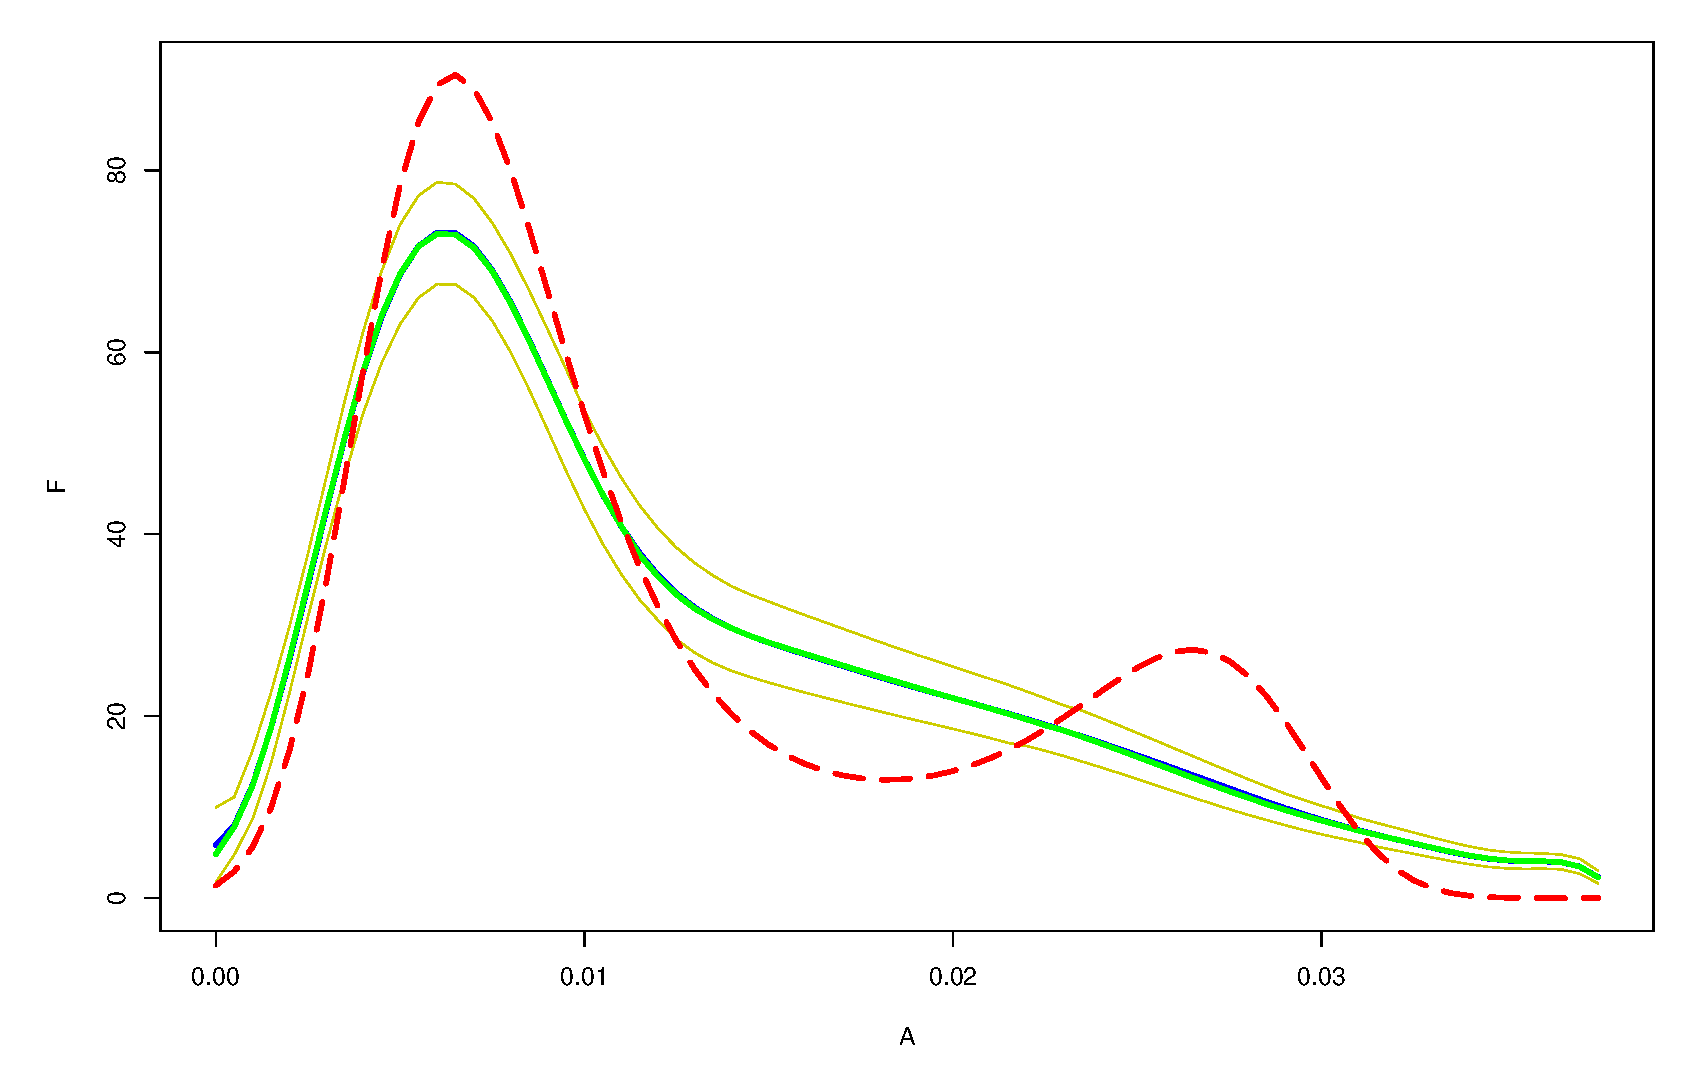
\includegraphics[width=0.5\linewidth]{example_fullbayesian.pdf}
%\caption{caption}\label{fig:comparison_a5}
\end{wrapfigure}% exp_family_maxent.nb
 analysis show that the most probable frequency distribution across recorded
bins (item i on p.~8) and the belief distribution over the total activity
at any recorded bin (item ii on p.~8) are visibly different. See figure on
the right: item (i) is the red dashed red curve, item (ii) the solid green
line.

Regarding the quantities mentioned on p.~8, it is important to know whether
we are calculating the frequency of past results, or the probability for a
new result, or the most probable frequency of future results. These
quantities can be numerically very different when the ratio
$\frac{\text{\# samples}}{\text{data-space dimension}}$ is high, and they
are to be used in different ways.

These are therefore not philosophical matters. It's a matter of
understanding and clearly stating what we are
calculating. % Unfortunately the
% neuroscience literature is very unclear on such matters.
There's also another important reason. We are generally concerned for
master's and PhD students, who often learn concepts and methods through
actual research, perusing works like the present one. Young researchers too
often end up learning incorrect or confused ideas, gathered from unclear
literature. % They trust it because it's peer-reviewed.
Sometimes the result, quoting Feynman \citey{feynman1985_r1989}, is that
\enquote{they don't learn by understanding; they learn by some other way --
  by rote, or something. Their knowledge is so fragile!}. We owe them
clarity, precision, honesty, and a glimpse of the bigger picture.



\addsec{Reviewer 2}
\label{sec:rev2}

2. {\footnotesize\textsf{\footnotesize The method requires that the
    measurements on n neurons are 'representative' of the full population
    of N neurons. The authors show one example, where they divide a dataset
    into two subsets of neurons with different statistics.  They show that
    the extrapolations from these two subsets are significantly different.
    But this particular analysis is somewhat ad hoc. Are there any more
    systematic tests of procedures for understanding how sensitive this
    analysis is to choosing different subsets of neurons? Or different
    recoding periods?}\par}

*** equiv to unsystematic sampling for extended recording arrays



3. {\footnotesize\textsf{\footnotesize In particular, correlations tend to be stronger between nearby neurons than far-away neurons. This should be a consistent pattern that shows up in most experimental datasets and which should lead to systematic biases in inferring the properties of populations, N, which are large enough to result in lower average correlation (see Nonnenmacher et al., PLoS CB 2017). Is there any way to take this dependence into account?}\par}

*** analogous to \enquote{design} in survey sampling


%%%% examples use empheq
%   \begin{empheq}[left={\mathllap{\begin{aligned}    \de\yF_{\yc}/\de\yp&=0\text{:} \\
%         \de\yF_{\yc}/\de\ym&=0\text{:}\\ \de\yF_{\yc}/\de\yl&=0\text{:}\end{aligned}}\qquad}\empheqlbrace]{align}
%     \label{eq:con_p}
% %    \de\yF_{\yc}/\de\yp &\equiv
%     -\ln\yp + \ln\yq + \yl\yM + \ym\yu &=0,\\
%     \label{eq:con_u}
% %    \de\yF_{\yc}/\de\ym &\equiv
%     \yu\yp-1 &=0,\\
%     \label{eq:con_l}
%     %\de\yF_{\yc}/\de\yl &\equiv
%     \yM\yp-\yc &=0.
%   \end{empheq}
%%%%
% \begin{empheq}[box=\widefbox]{equation}
%   \label{eq:maxent_question}
%   \p\bigl[\yE{N+1}{k} \bigcond \tsum\yo\yf{N}\in\yA, \yM\bigr] = \mathord{?}
% \end{empheq}



% \[
%   \begin{tikzcd}
%       M_{n,n}(\CC) \arrow{r}{R'_{a}(\Hat{U})} & M_{n,n}(\CC)
%     \\
%     L(\mathcal{H}) \arrow{r}{\Hat{U}} \arrow[swap]{d}{R_*}\arrow[swap]{u}{R'_*} & L(\mathcal{H}) \arrow{d}{R_*}\arrow{u}{R'_*} \\
%       M_{n,n}(\CC) \arrow{r}{R_{a}(\Hat{U})} & M_{n,n}(\CC)
%   \end{tikzcd}
% \]

% \[
%   \begin{tikzcd}
%       \CC^n \arrow{r}{R'_*(A)} & \CC^n
%     \\
%     \mathcal{H} \arrow{r}{A} \arrow[swap]{d}{R}\arrow[swap]{u}{R'} & \mathcal{H} \arrow{d}{R}\arrow{u}{R'} \\
%       \CC^n \arrow{r}{R_*(A)} & \CC^n
%   \end{tikzcd}
% \]


% \[
%   \begin{tikzcd}
%     \mathcal{H} \arrow{r}{A} \arrow[swap]{d}{R} & \mathcal{H} \arrow{d}{R} \\
%       \CC^n \arrow{r}{R_*(A)} & \CC^n
%   \end{tikzcd}
% \]

%%\setlength{\intextsep}{0.5ex}% with wrapfigure
%\begin{figure}[p!]%{r}{0.4\linewidth} % with wrapfigure
%  \centering\includegraphics[trim={12ex 0 18ex 0},clip,width=\linewidth]{maxent_saddle.png}\\
%\caption{caption}\label{fig:comparison_a5}
%\end{figure}% exp_family_maxent.nb


%%%%%%%%%%%%%%%%%%%%%%%%%%%%%%%%%%%%%%%%%%%%%%%%%%%%%%%%%%%%%%%%%%%%%%%%%%%%
%%% Acknowledgements
%%%%%%%%%%%%%%%%%%%%%%%%%%%%%%%%%%%%%%%%%%%%%%%%%%%%%%%%%%%%%%%%%%%%%%%%%%%% 
\iffalse
\begin{acknowledgements}
  \ldots to Mari \amp\ Miri for continuous encouragement and affection, and
  to Buster Keaton and Saitama for filling life with awe and inspiration.
  To the developers and maintainers of \LaTeX, Emacs, AUC\TeX, Open Science
  Framework, R, Python, Inkscape, Sci-Hub for making a free and impartial
  scientific exchange possible.
%\rotatebox{15}{P}\rotatebox{5}{I}\rotatebox{-10}{P}\rotatebox{10}{\reflectbox{P}}\rotatebox{-5}{O}.
%\sourceatright{\autanet}
\mbox{}\hfill\autanet
\end{acknowledgements}
\fi

%%%%%%%%%%%%%%%%%%%%%%%%%%%%%%%%%%%%%%%%%%%%%%%%%%%%%%%%%%%%%%%%%%%%%%%%%%%%
%%% Appendices
%%%%%%%%%%%%%%%%%%%%%%%%%%%%%%%%%%%%%%%%%%%%%%%%%%%%%%%%%%%%%%%%%%%%%%%%%%%% 
\bigskip
% %\renewcommand*{\appendixpagename}{Appendix}
% %\renewcommand*{\appendixname}{Appendix}
% %\appendixpage
% \appendix

%%%%%%%%%%%%%%%%%%%%%%%%%%%%%%%%%%%%%%%%%%%%%%%%%%%%%%%%%%%%%%%%%%%%%%%%%%%%
%%% Bibliography
%%%%%%%%%%%%%%%%%%%%%%%%%%%%%%%%%%%%%%%%%%%%%%%%%%%%%%%%%%%%%%%%%%%%%%%%%%%% 
\renewcommand*{\finalnamedelim}{\addcomma\space}
\defbibnote{prenote}{{\footnotesize (\enquote{de $X$} is listed under D,
    \enquote{van $X$} under V, and so on, regardless of national
    conventions.)\par}}
% \defbibnote{postnote}{\par\medskip\noindent{\footnotesize% Note:
%     \arxivp \mparcp \philscip \biorxivp}}

\printbibliography[%prenote=prenote%,postnote=postnote
]

\end{document}

%%%%%%%%%%%%%%%%%%%%%%%%%%%%%%%%%%%%%%%%%%%%%%%%%%%%%%%%%%%%%%%%%%%%%%%%%%%%
%%% Cut text (won't be compiled)
%%%%%%%%%%%%%%%%%%%%%%%%%%%%%%%%%%%%%%%%%%%%%%%%%%%%%%%%%%%%%%%%%%%%%%%%%%%% 


%%% Local Variables: 
%%% mode: LaTeX
%%% TeX-PDF-mode: t
%%% TeX-master: t
%%% End: 
